\newpage
\section{La France et la DGSE}

\newthought{La France a} elle aussi une longue tradition dans le chiffre, et ses
services de renseignement extérieur font partie des meilleurs du monde.
Contrairement au Royaume-Uni et à l'Allemagne, elle dispose de gros moyens
propres, et n'a donc pas une tradition de coopération avec la NSA aussi forte
que ses voisins. 

\newthought{En effet,} de part la présence d'un opérateur de catégorie mondiale
sur son territoire (Orange) ainsi que de différents points d'arrivées de câbles
sous-marins (Marseille pour le Proche-Orient notamment), la France est à un
carrefour stratégique des autoroutes numériques. La DGSE l'a bien compris, et
opère dans ses locaux parisiens le second plus gros programme de surveillance
européen, après celui des anglais\ldots\cite{DGSE}

\newthought{Pas franchement légal,} ce programme est soupçonné d'avoir été
complété par des installations\cite{reflets} d'équipements fournis par une
société \emph{française} spécialisée dans la technique dite de DPI\footnote{Deep
Packet Inspection :
l'analyse des flux de données en profondeur}, Amesys (filiale du géant français
Bull\ldots).
Cette dernière a fait l'objet d'une très longue saga d'articles publiés chez les journalistes d'investigation de
Reflets.info, et il n'est pas inutile d'aller lire la centaine de documents
publiés pour se rendre compte de la complexité de la chose.

\newthought{Il serait trop} long de faire un descriptif exhaustif des faits,
mais on peut retenir plusieurs choses :

\begin{itemize}
  \item Amesys a vendu un de ses produit d'interception de masse (au niveau
  d'un pays), EAGLE, au régime totalitaire de Kadhafi\cite{libye}
  \item Amesys est actuellement en train d'installer le même équipement au
  Maroc\cite{maroc}, ce qui inquiète fortement les opposants au régime
  marocain, déjà fortement réprimés.
  \item Qosmos, un autre leader du DPI et lui aussi français, a vendu des
  sondes d'inspection au régime de Bachar al-Assad en Syrie\cite{qosmos}
  \item Une plainte a été déposée par la FIDH pour << complicité de crimes de
  torture >> contre Qosmos et Amesys devant le Parquet de Paris.\cite{fidh}
\end{itemize}

\newthought{Ces faits sont} d'autant plus troublants que la société Elexo, soeur
d'Amesys, vient de candidater\cite{elexo} pour le marché public ouvert pour la
nouvelle Loi sur le Renseignement, votée il y a peu, et instaurant la mise en place de <<
boîtes noires >> sur les coeurs de réseau de l'Internet français\cite{LR} (du
DPI légal, en somme).

\newpage
\subsection{Frenchelon}

\newthought{Contraction des termes} <<~French~>> et <<~ECHELON~>>, ce nom
désigne les stations d'écoutes opérées sur le territoire national par la
DGSE\footnote{Direction Générale de la Sécurité Extérieure, les services secrets
français} et la DRM\footnote{Direction du Renseignement Militaire, la branche
en charge des renseignements au sein de l'Armée.}. Il en existerait une
quinzaine, dont la plus importante se situe à Domme :

\vspace{0.7cm}
\begin{figure}
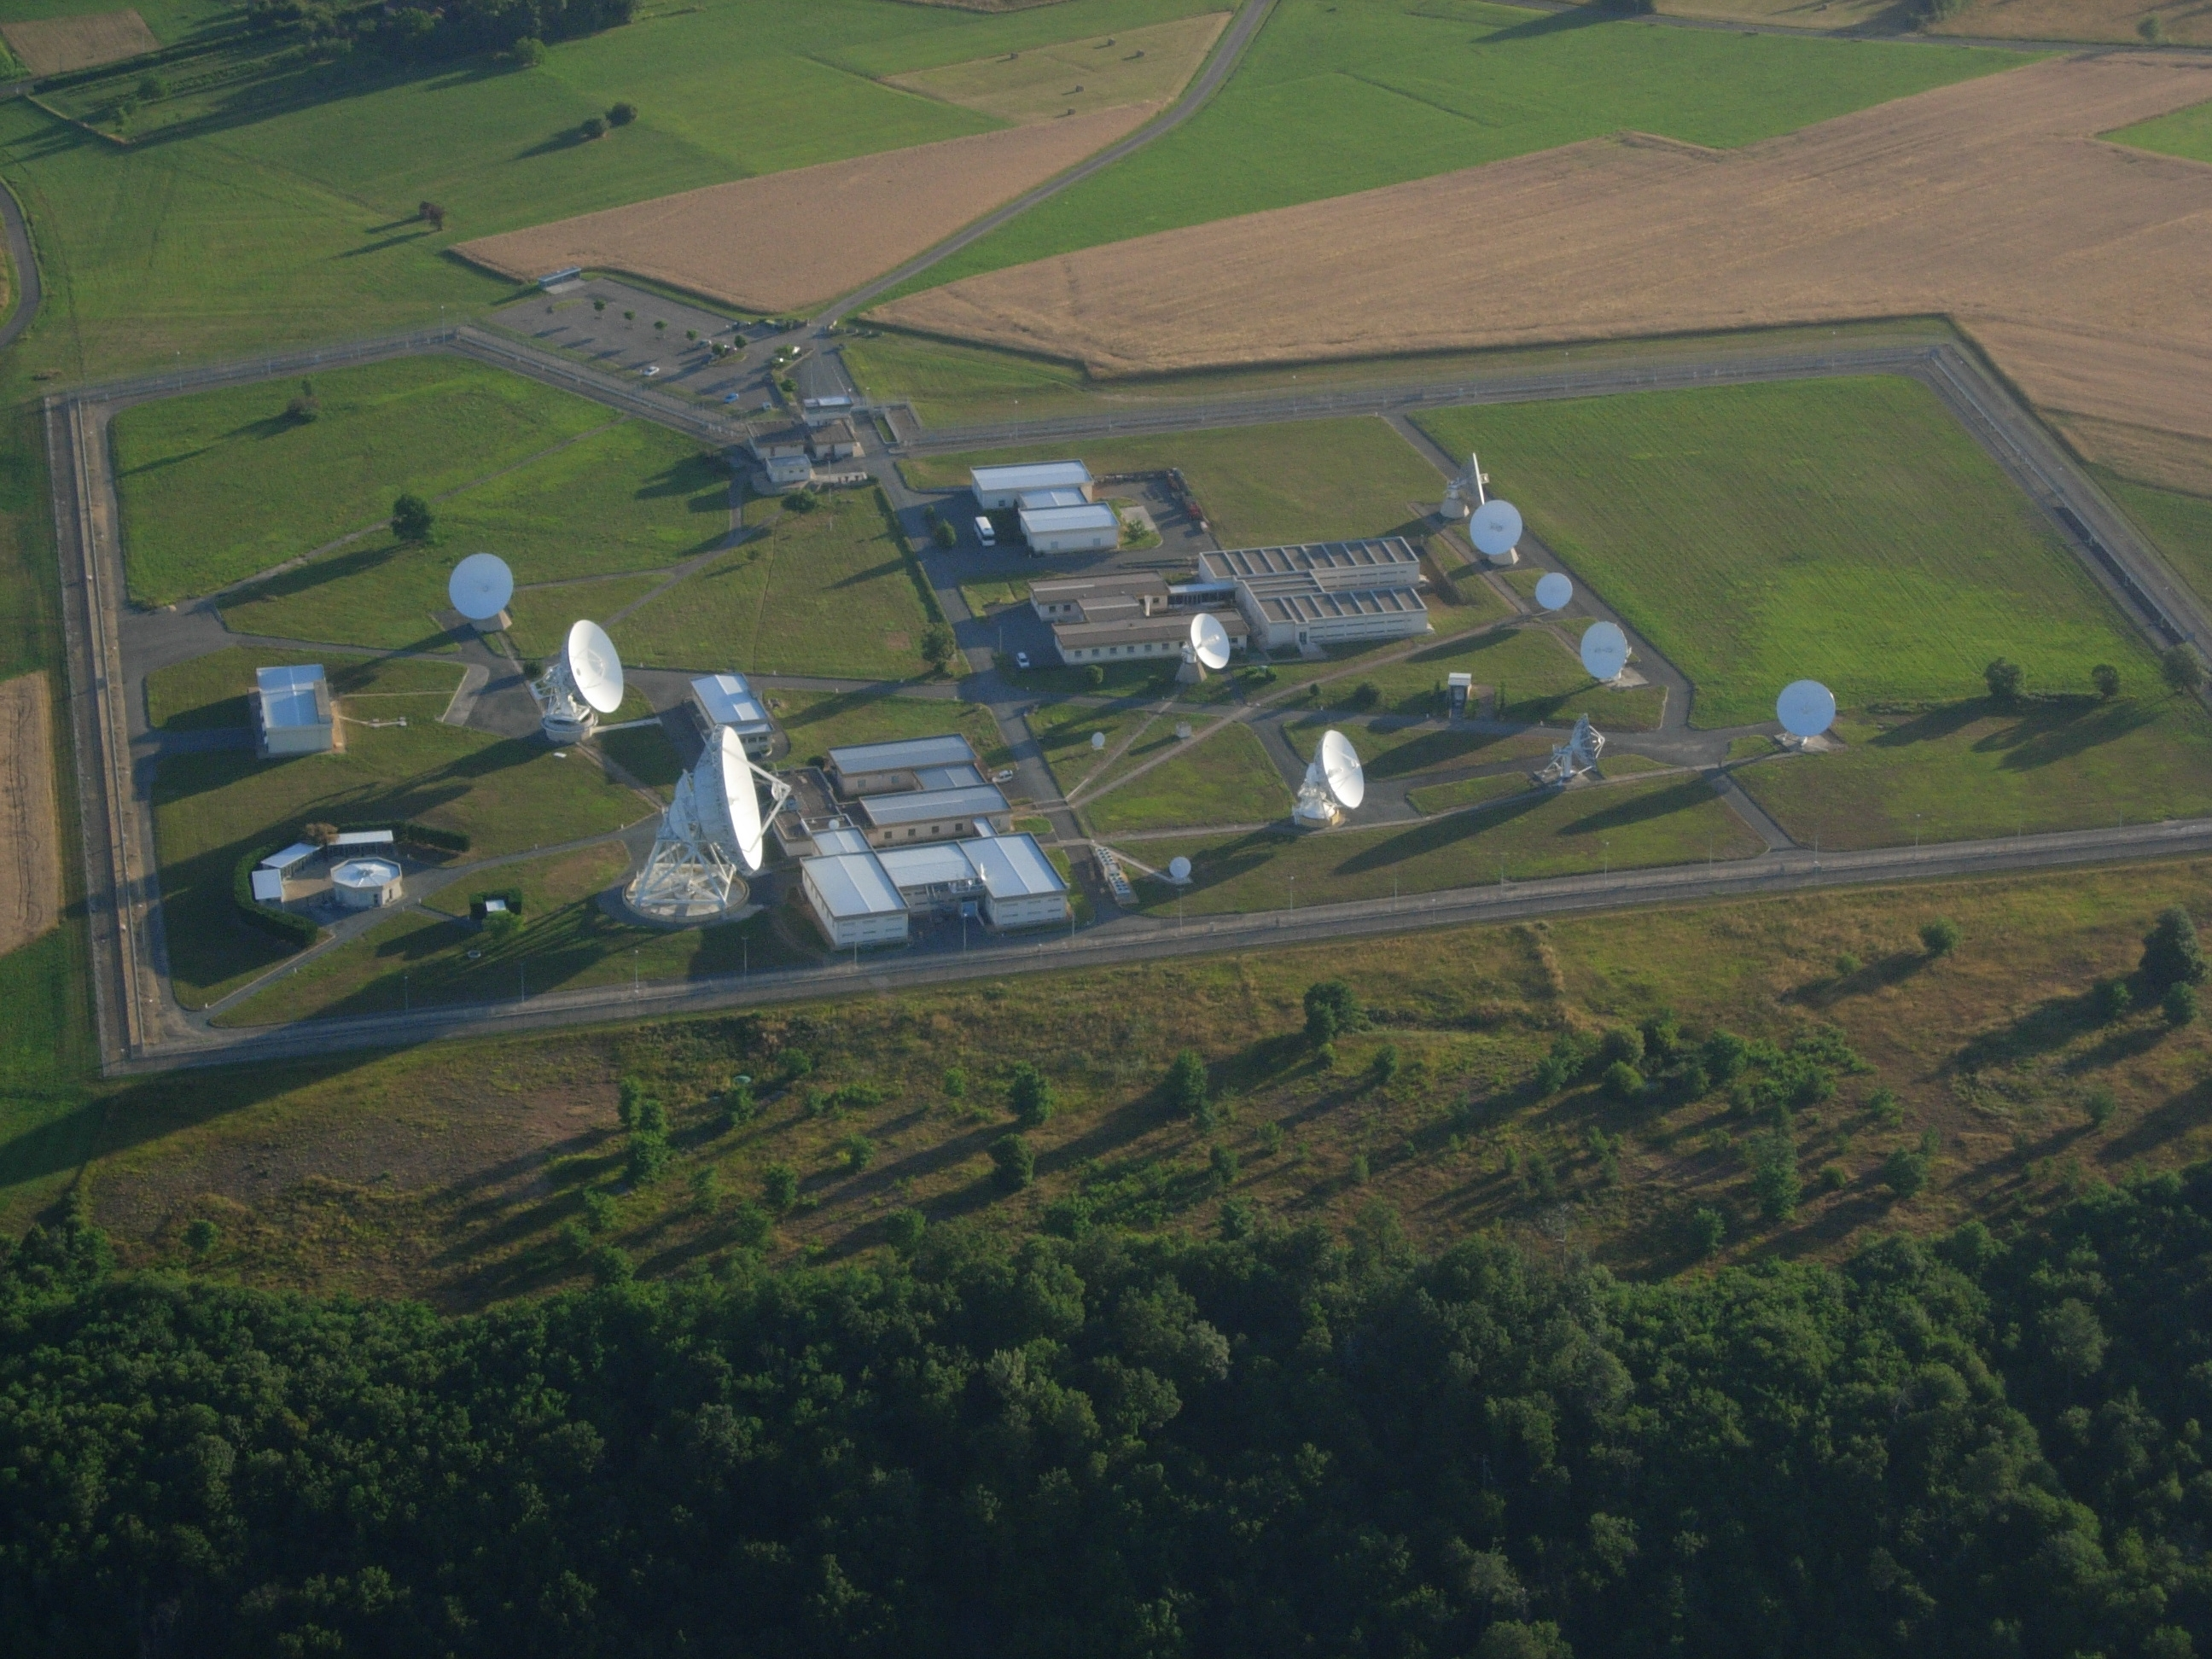
\includegraphics{french1.jpg}
\caption[Station d'écoute de Domme][6pt]{Station d'écoute de la DGSE
à Domme}
\label{fig:french1}
\end{figure}


\newthought{Tout comme ECHELON,} le programme français permet d'intercepter de
grandes quantités de données sur tout le spectre électromagnétique, afin d'être
analysées plus tard. Ces données peuvent être ensuite utilisées par tous les
acteurs du renseignement en France, et sont stockées dans les locaux parisiens
de la DGSE.\cite{bbf}

\newthought{Les technologies utilisées} par ce programme sont en partie issues
d'appels d'offres de la DGA et de développements assurés par EADS (aujourd'hui
Airbus Defence And Space), notamment le système HERISSON\footnote{Habile
extraction du renseignement d'intérêt stratégique à partir de sources ouvertes
numérisées}\cite{herisson} en charge de l'extraction de renseignements en
sources ouvertes (réseaux sociaux, Internet, etc).

\newpage
\subsection{L'accord LUSTRE}

\newthought{Derrière ce nom} se cache l'accord d'échange de données
interceptées signé entre la DGSE pour la partie française et la NSA pour la
partie américaine. C'est l'équivalent de l'accord UKUSA, mais contrairement à ce
dernier, très peu d'informations sont disponibles sur les modalités de l'accord.

\newthought{L'accord fut signé} fin 2011\cite{lustre}, et permet à la France
d'accéder aux données de la NSA sur des parties du monde où ses capacités de renseignement
sont limitées, tandis qu'elle fournit à la NSA des données sur lesquelles la
France dispose de bonnes connexions (voir figure \ref{fig:french2}), notamment
le Proche-Orient et l'Afrique (il y a environ trente fois plus de trafic Afrique -> Europe qu'Afrique ->
\EUA).

\vspace{0.7cm}
\begin{figure}
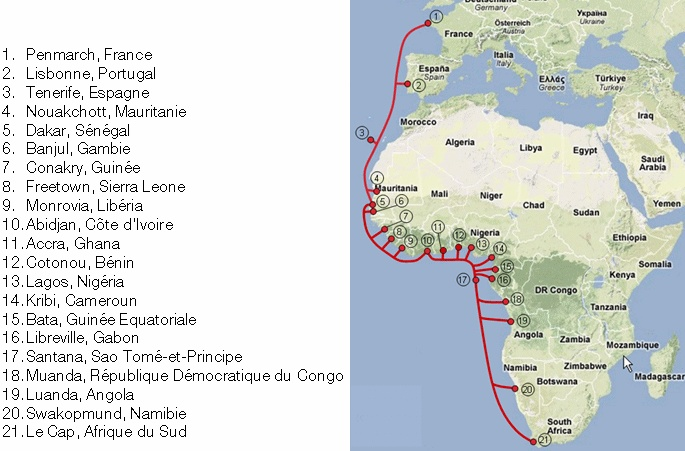
\includegraphics{french2.jpg}
\caption[Câble sous-marin reliant l'Afrique à l'Europe][6pt]{Câble sous-marin
reliant l'Afrique à l'Europe}
\label{fig:french2}
\end{figure}

\newthought{Ces informations expliquent} en partie le relatif silence des
autorités françaises à propos des révélations d'Edward Snowden, puisqu'elle se
permet de faire exactement la même chose de son côté. Il
est d'ailleurs intéressant de noter que l'accord LUSTRE fut révélé au public par
le Général Keith Alexander\footnote{La directeur de la NSA de l'époque} lors
d'une audition devant la commission de renseignement américaine, après que les pays
européens, dont la France, ont commencé à protester contre les révélations
faites sur PRISM. Faites ce que je dis\ldots